% !TEX root = talk.tex
\begin{frame}[t]{Definition}
\begin{block}{Dirichlet Process (DP), \citet{Ferguson1973}}
We say
 \[G \sim \DP(c,G_0)\]
 if for any partition $A_1, \ldots, A_k$ of the sample space, the vector of random probabilities
$[G(A_1), \ldots, G(A_k)]$ follows a Dirichlet distribution, i.e.
\[[G(A_1), \ldots, G(A_k)] \sim \Dir(cG_0(A_1), \ldots, cG_0(A_k))\]
\end{block}
\end{frame}	

\begin{frame}[t]{Properties}
\begin{block}{Basics}
\begin{eqnarray*} 
[G(A),G(A^C)] \sim \Dir(cG_0(A), cG_0(A^C)) 
\end{eqnarray*}
reduces to
\[G(A) \sim \Bet(cG_0(A), cG_0(A^C))\]
which means
\[ \Ave(G(A)) \comment{= \frac{cG_0(A)}{cG_0(A)+cG_0(A^C)}} = G_0(A)\] 
and
 \begin{eqnarray*} 
\Var(G(A)) &=& \comment{\frac{c^2G_0(A)G_0(A^C)}{(cG_0(A)+cG_0(A^C))^2(cG_0(A)+cG_0(A^C)+1)} \\
&=&} \frac{G_0(A)(1-G_0(A))}{(c+1)}
 \end{eqnarray*}
\end{block}
 Note, as $c\rightarrow\infty, \Var(G(A))\rightarrow0$ and thus $G(A) \rightarrow G_0(A)$
\end{frame}	

\begin{frame}[t]{Explicit Construction}
\begin{block}{\citet{Sethuraman1994a}}
\[G(\cdot) = \sum_{k=1}^\infty w_k \delta_{\phi_k}(\cdot)\]
where 
\[{\phi_k} \sim G_0 \mbox{ and } w_k = V_k\prod_{j<k}(1-V_j), V_k \sim \Bet(1,c)\]
\end{block}
Note: this is known as the ``stick-breaking'' construction.
\end{frame}	

\begin{frame}[t]{Efficient Posterior Updating}
\begin{block}{Polya Urn \citep{Blackwell1973}}
\begin{eqnarray*}
x_1 &\sim& G_0 \\
G | x_1 &\sim& \DP\left(1+c, \frac{1}{1+c}\delta_{x_i} + \frac{c}{1+c}G_0\right)\\
x_2 | x_1 &\sim& \frac{1}{1+c}\delta_{x_i} + \frac{c}{1+c}G_0 \\
G | x_1, x_2 &\sim& \DP\left(2+c, \frac{1}{2+c}\sum_{i=1}^n \delta_{x_i} + \frac{c}{2+c}G_0\right)\\
&\vdots&\\
\end{eqnarray*}
\end{block}
\end{frame}	


\begin{frame}[t]{Efficient Posterior Updating}
\begin{block}{Polya Urn \citep{Blackwell1973} Cont.}
\begin{eqnarray*}
x_n | x_1,\ldots x_{n-1} &\sim& \frac{1}{n-1+c}\sum_{i=1}^{n-1}\delta_{x_i} + \frac{c}{n-1+c}G_0 \\
G | x_1, \ldots, x_n &\sim& \DP\left(n+c, \frac{1}{n+c}\sum_{i=1}^n \delta_{x_i} + \frac{c}{n+c}G_0\right)
\end{eqnarray*}
Note: 
\begin{itemize}
\item Neither posterior predictive nor posterior distributions depend on the order of the $x_i$'s ($x_i$'s ``exchangeable'')
\item Many $x_i$'s will share the same value, call a shared value $\phi_k$
\item ``Observing'' $\phi_k$ once increases probability of observing it again and this is reinforced
\end{itemize}
\end{block}
\end{frame}	

\begin{frame}[t]{Incremental Estimation}
\begin{block}{Sequential Monte Carlo}
The posterior distribution is fully characterized by 
\[\frac{1}{n-1+c}\sum_{i=1}^{n-1}\delta_{x_i} + \frac{c}{n-1+c}G_0\]
Particle filters for posterior estimation in general DP models can be constructed by, for each new observation either
\begin{itemize}
\item {\em Sampling}
\item {\em Enumerating} 
\end{itemize}
whether the observation arose from
\[\frac{1}{n-1+c}\sum_{i=1}^{n-1}\delta_{x_i}  \quad \mbox{      or        } \quad \frac{c}{n-1+c}G_0\]
\end{block}
\end{frame}

\begin{frame}[t]{Incremental Estimation}
\begin{block}{Sequential Monte Carlo}
In the discrete likelihood case, an ``efficient''  {\em single}-particle particle filter posterior estimator consists of a particle $\ell = 1$ containing a set of draws from the base distribution 
\[\Phi_\ell = \{\phi_k\}_{k=1}^K, \phi_k \sim G_0\]
and a set of counts, one per $\phi_k$, indicating how many times each draw from the base distribution was responsible for generating an observation
\[{\bf c}_\ell = \{c_k\}_{k=1}^K\]
\end{block}
Note, $K\leq N$
\end{frame}

\begin{frame}[t]{Uses}
\begin{block}{Density Estimation, Mixing A Smooth Kernel}
Dirchlet Process Mixture model \citep{Escobar1995, MacEachern1998, Neal1998}
\begin{eqnarray*}
G &\sim& \DP(c,G_0) \\
\theta_i &\sim& G \\
x_i | \theta_i &\sim& F(\theta_i),
\end{eqnarray*} 
or equivalently%
\begin{eqnarray*}
z_i &\sim& \CRP(c) \\
\theta_k &\sim& G_0 \\
x_i | z_i &\sim& F(\theta_{z_i})
\end{eqnarray*} 

\end{block}

Note: constructing SMC or MCMC samplers for either of these representations is more complicated but still straightforward.
\end{frame}	


\begin{frame}[t]{Uses}
\begin{block}{Hierarchical Dirichlet Process \cite{Teh2006b}}
Dirichlet processes can be used as ``glue'' to hierarchically tie together distributions governing related populations in order to ``share statistical strength'' during inference.
\begin{columns}[t]
\begin{column}{.5\textwidth}
\begin{eqnarray*}
G &\sim& \DP(c,G_0) \\
G_j &\sim& \DP(c,G) \\
\theta_{ij} &\sim& G_j \\
x_{ij} | \theta_{ij} &\sim& F(\theta_{ij}),
\end{eqnarray*} 
\centering
\hspace{.25cm} here $G_j$ is a per-class distribution over population {\em parameters}.
\vspace{2cm}
\end{column}
\begin{column}{.5\textwidth}
\begin{figure}
\begin{center}
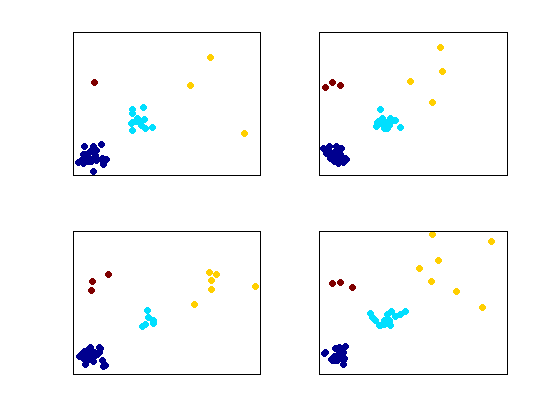
\includegraphics[trim = 4cm 8cm 4cm 8cm, clip, width=5cm]{fig/shared_clustering.pdf}
%\caption{Shared clustering}
\label{default}
\end{center}
\end{figure}
\end{column}
\end{columns}
\end{block}
\end{frame}	


\begin{frame}[t]{Hierarchical Dirichlet Process Inference}
%SMC and MCMC algorithms based on the Polya urn representation exist for hierarchical DP's as well.  
Consider the ``full characterization'' of the posterior predictive distribution of the base level of a DP model
\begin{eqnarray*}
G &\sim& \DP(c,G_0) \\
G_j &\sim& \DP(c,G) \\
\theta_{ij} &\sim& G_j \\
\end{eqnarray*} 
i.e.
\[\theta_{nj} | \theta_{1j}, \ldots, \theta_{n-1,j} =  \frac{1}{n-1+c}\sum_{i=1}^{n-1}\delta_{\theta_{ij}} + \frac{c}{n-1+c}G_j\]

\end{frame}

\begin{frame}[t]{Hierarchical Dirichlet Process Inference}
Now consider $G_j$ as having been similarly marginalized out and represented in the same way

\[\psi_{nj} | \psi_{1j}, \ldots, \psi_{n-1,j} =  \frac{1}{n-1+c}\sum_{i=1}^{n-1}\delta_{\psi_{ij}} + \frac{c}{n-1+c}G\]
Consider the following argument.  If $\theta_{nj} \notin \{\theta_{ij}\}_{i=1}^{n-1}$ then $\theta_{nj}$ must be explained as having been a draw from the base distribution $G_j$
\[\theta_{nj} | \theta_{1j}, \ldots, \theta_{n-1,j} =  \frac{1}{n_j-1+c}\sum_{i=1}^{n_j-1}\delta_{\theta_{ij}} + \frac{c}{n_j-1+c}G_j\]
and correspondingly there must be some $\psi_{ij} = \theta_{ij}$.  This could be one of the existing $\psi$'s or a draw from $G$. This intuition is the basis for MCMC and SMC HDP samplers.  


\end{frame}